\chapter{Qualitätssicherung}
\label{chap:Qualitätssicherung}
Die Qualität des Source-To-Source Compilers muss während und nach der erfolgreichen Implementierung sichergestellt werden.  Im ersten Abschnitt dieses Kapitels erfolgt die Vorstellung der Komponententests als Qualitätssicherungsmaßnahme im Verlauf der Entwicklung.  Anschließend wird die Funktionsweise des Compilers mithilfe einer speziell entwickelten Xamarin.Forms App überprüft.  Anhand dieser Maßnahmen kann  festgestellt werden,  ob der Compiler erwartungsgemäß arbeitet. 

\section{Komponententests}
Komponententests unterteilen ein Programm in einzelne,  testfähige Einheiten und validieren deren Funktionalität.  Wenn sie integraler Bestandteil des Entwicklungspozesses sind,  optimieren sie die Qualität des Programms.  In Visual Studio können diese Testfälle bei Änderungen am Quelltext automatisiert durchgeführt werden, was garantiert, dass die Modifikation am Code kein unerwünschtes Verhalten erzeugt.   Sobald eine Klasse oder Methode geschrieben ist, beginnt die Analyse, die das Verhalten des Codes nach Eingabe von gültigen, falschen und grenzwertig gültigen Daten überprüft. \footcite[Vgl.][Abgerufen am \today]{MicrosoftColor}  Diese testgesteuerte (engl. testdriven) Entwicklung entspricht der Qualitätssicherung bei 
der Programmierung des Source-To-Source Compilers, denn auch hier wurden die Komponententests vor dem Quelltext geschrieben und dienen damit  der funktionalen Spezifikation der Anforderungen.

Dieses Testverfahren soll exemplarisch anhand der Umwandlung von Farben veranschaulicht 
werden.
App-Entwickler können die Farbe mit einem gültigen Farbnamen oder als Hexadezimalzahl 
angeben. Hexadezimale Darstellungen können jeweils über drei, vier, sechs oder acht Ziffern mit
einem optionalen Präfix \# angegeben werden.  \footcite[Vgl.][Abgerufen am \today]{MicrosoftColor} 
Diese verschieden verfügbaren Eingabeformate machen es notwendig, dass der Compiler eine 
vollständige Umwandlung vornimmt.  
Anhand dieser Anforderungen können nun die in Quelltext \ref{lst:colorTest} gezeigten Testfälle entworfen werden.

\lstinputlisting[label={lst:colorTest},caption={Testfälle für die Umwandlung von Farben}, language=csh]{SourceCode/Testcases.cs}

Durch die im Quelltext aufgeführten Komponententests kann nun der in Quelltext \ref{lst:colorTestAlgo} dargestellte Algorithmus realisiert werden. 
\newpage
\lstinputlisting[label={lst:colorTestAlgo},caption={Algorithmus für die Umwandlung von Farben}, language=csh]{SourceCode/AlgorithmusColor.cs}


\section{Manuelles Testing}
Die weiterführende Qualitätssicherung des Compilers macht es erforderlich,  neben den Komponententests auch ein manuelles Testing vorzunehmen. Hierfür wird ein Testobjekt entwickelt und kompiliert, bevor anhand von manuellen Arbeitsschritten die Quell- und Zielobjekte verglichen werden.

\subsection{Testobjekt}
Die Testapp wurde mit der Version 5.0.0.2012 des Xamarin.Forms Frameworks realisiert und verwendet die Erweiterungen Xamarin.Essentials.  Als Testobjekt soll diese mobile Anwendung möglichst viele Funktionalitäten von Xamarin.Forms abbilden,  hat jedoch nicht den Anspruch einer vollständigen Testabdeckung.
Auf plattformspezifische Implementationen mit Ausnahme der Metadaten und Ressourcen wurde verzichtet.  Eine genaue Beschreibung der App-Funktionalitäten und -Eigenschaften folgt und wird mithilfe von iOS Screenshots veranschaulicht.  Die entsprechenden Android Screenshots befinden sich in \hyperref[chap:AnhangAndroidScreenshots]{Anhang III}.  

Abbildung \ref{fig:TestObjectI} zeigt im ersten Screenshoot den Startbildschirm mit dem Namen und Icon der Testapp und im zweiten den Hauptbildschirm.  


\begin{figure}[!ht]
 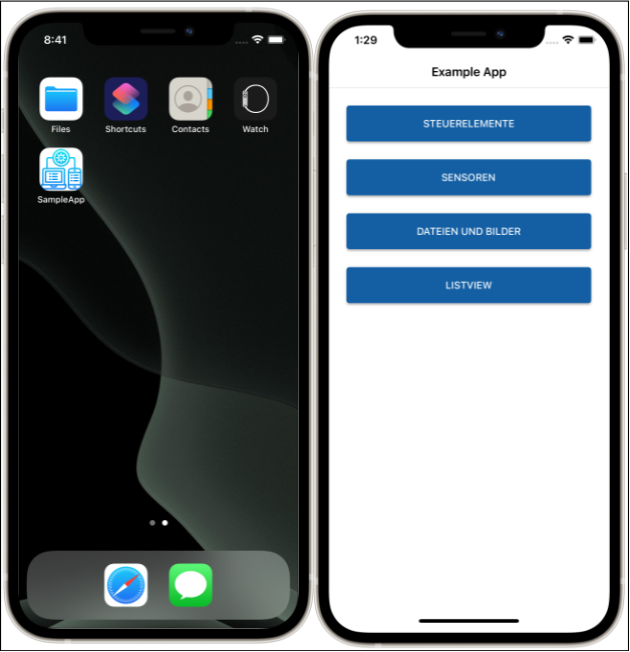
\includegraphics[width=\textwidth,keepaspectratio]{Images/Screenshot/AppIconAndMenu.png}
 \caption{Test Objekt Screenshots I}
 \label{fig:TestObjectI}
\end{figure}

Anhand des Namens (SampleApp) und eines Anwendungsicons können Anwender die App auf dem Startbildschirm identifizieren.  Nach ihrem Start öffnet sich eine Menüstruktur,  die Wurzel der Navigation, über die verschiedene Bereiche der mobilen Anwendung angesteuert werden können.  In einer vertikalen Ansicht werden dafür Schaltflächen als Ereignisauslöser für die Navigation bereitgestellt,  die zu den Seiten: \glq Übersicht der Steuerelemente\grq ,  \glq Ausgabe von Smartphonesensoren\grq ,  \glq Arbeit mit Bildern\grq{}  und \glq Ansicht einer Listview\grq{}  führen.  
Abbildung \ref{fig:TestObjectII} zeigt die Übersicht der Steuerelemente sowie die Werte der Smartphone-Sensoren.

\begin{figure}[!ht]
 \includegraphics[width=\textwidth,keepaspectratio]{Images/Screenshot/Sensors.png}
 \caption{Test Objekt Screenshots II}
 \label{fig:TestObjectII}
\end{figure}
Die Darstellung visualisiert die gängigsten Steuerelemente,  die anhand der in Kapitel 4 aufgeführten Kategorien gruppiert und vertikal angeordnet wurden.  Zu den in der App angezeigten Elementen gehören unter anderem eine Schaltfläche,  ein Bild und im Screenshot nicht erkennbar Auswahlmöglichkeiten für Datum und Uhrzeitwerte.  Der zweite Screenshot zeigt eine Übersicht der aktuellen Werte des Beschleunigungssensors und des Gyroskopes,  die beide über das Plugin Xamarin.Essentials in der Codebehind-Datei ausgelesen und über Databindings im \ac{ui} angezeigt werden.    

Die nächsten beiden Screenshots in \ref{fig:TestObjectIII} visualisieren das Menü für die Arbeit mit Bildern und einen zusätzlichen Berechtigungsdialog rechts.

 
\begin{figure}[!ht]
 \includegraphics[width=\textwidth,keepaspectratio]{Images/Screenshot/Permissions.png}
 \caption{Test Objekt Screenshots III}
 \label{fig:TestObjectIII}
\end{figure}
Das Menü hat Ähnlichkeiten mit dem der Hauptseite.  Statt einer Navigation werden hier jedoch plattformspezifische Funktionalitäten über das Xamarin.Essentials Plugin ausgeführt, die einen Zugriff auf die Kamera und die Galerie des Smartphones bieten.  Der Dialog,  der nach der Zugriffsberechtigung fragt, zeigt in der iOS Version einen Eintrag aus den Metadaten an.
Die nächste Abbildung stellt im linken Screenshot die Auswahlfunktion von Bildern aus der Galerie dar und rechts eine ListView mit Namen und E-Mail-Adressen von fiktiven Benutzern.  
Die Klasse \glq Benutzer\grq{} wird innerhalb des Quelltextes der mobilen Anwendung definiert und über den Namespace in der Codebehind-Datei referenziert.  Anschließend werden exemplarisch zehn Objekte dieser Klasse innerhalb der Codebehind Datei  in Form einer Auflistung vorgehalten und mithilfe eines Databindings in der ListView angezeigt. 
 
\begin{figure}[!ht]
 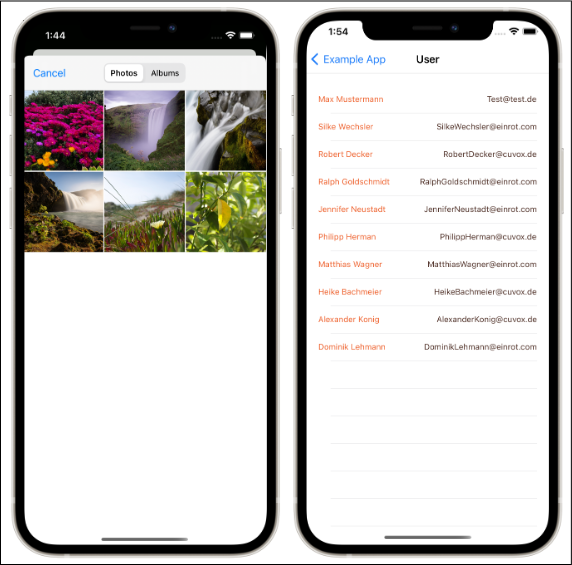
\includegraphics[width=\textwidth,keepaspectratio]{Images/Screenshot/ImagesListView.png}
 \caption{Test Objekt Screenshots IV}
 \label{fig:TestObjectIV}
\end{figure}


\subsection{Testfälle}
Zur Überprüfung der Funktionalität des Compilers müssen Testfälle definiert werden,  mit denen die übersetzte mobile Anwendung manuell validiert wird.  Relevante Prüfobjekte lassen sich sowohl aus dem visuellen  Erscheinungsbild als auch aus dem Funktionsspektrum des Testobjekts ableiten und sind in Tabelle \ref{tab:Testapp} aufgeführt.  Dieser Testkatalog kann erweitert werden,  ist jedoch für eine Qualitätssicherung zur Beantwortung der Forschungsfrage ausreichend.  
\newpage

\begin{table}[!ht]
\begin{tabularx}{\textwidth}{|l|X|}
\hline
 \textbf{Prüfobjekt} & \textbf{Prüfvorgang}  \\  
\hline
App-Icon	           					& Wird das App-Icon übernommen                       			 		\\ 
App-Name          					& Wird der App-Name übernommen                      		 \\ 
Seitenname  	         				& Wird in der Navigationsleiste der Name der aktuellen Seite angezeigt               \\ 
Menü         			  				& Werden alle 4 Menüpunkte angezeigt                     			 \\ 
Navigation         			  		& Wird mithilfe des Menüs navigiert	\\ 
Navigation          					& Wird über die \glq Zurück-Schaltfläche\grq{} in der Navigationsleiste zurück zur letzten Seite navigiert                   			 \\ 
Schriftgrößen			         	& Werden  Schriftgrößen korrekt übernommen                 			 \\ 
Farben						         	& Werden  Farben korrekt übernommen                 			 \\ 
Layouts 								& Werden alle Layouts durch die entsprechenden Widgets ersetzt              			 \\ 
Steuerelemente						& Werden alle Steuerelemente durch die entsprechenden Widgets ersetzt               			 \\ 
Beschleunigungssensor        	& Werden die Werte des Beschleunigungssensors ausgelesen          			 \\ 
Gy­ro­s­kop						         & Werden die Werte des Gyroskopes ausgelesen                            			 \\ 
Kamera			         				& Können Bilder über die Kamera aufgenommen werden\\ 
Galerie			         				& Können Bilder aus der Galerie ausgewählt werden                			 \\ 
Berechtigungen			         	& Wird beim Zugriff auf Kamera und Galerie nach einer Zugriffsberechtigung gefragt \\ 
ListView					         	& Werden in der Listview die generierten Daten angezeigt                   			 \\ 
\hline
\end{tabularx}
	  \caption{Testfälle zur Qualitätssicherung}
 \label{tab:Testapp}
\end{table}

\subsection{Testablauf}
In diesem Abschnitt werden die genannten Testfälle durchgeführt und ihr Ergebnis dokumentiert.
Der Start  des Testlaufs beginnt mit dem Aufruf der \ac{gui},  der Auswahl der Xamarin.Forms Testapp und eines leeren Ordners, der als Zielverzeichnis nach der Kompilierung dient. 
Aufgrund der vielen Dateizugriffe und durchzuführenden Aktionen nimmt die Übersetzung der Anwendung eine gewisse Zeit in Anspruch. Im Frontend lassen sich Informationen über den Status, den Verlauf und mögliche Fehlerquellen nach der Übersetzung ablesen.  Anschließend kann die fertige Flutter Anwendung mithilfe der SDK kompiliert und ihre Ansichten kontrolliert werden.  Die im Folgenden visualisierten Screenshots zeigen die generierte iOS Flutter-App,  die entsprechenden Androidrepräsentationen befinden sich in  \hyperref[chap:AnhangAndroidScreenshotsFlutter]{Anhang IV} dieser Arbeit.  Die Screenshots der übersetzten App zeigen die gleichen Bildschirmstatus wie die der Ausgangsapp, um eine Vergleichbarkeit zu gewähren.  Das nahezu identische Erscheinungsbild lässt bereits auf den ersten Blick eine hohe Qualität des Prototypen vermuten.  

In Abbildung \ref{fig:FlutterAppI} wird links der Startbildschirm mit dem Namen und Icon und rechts das zentrale Menü der App dargestellt. 

\begin{figure}[!ht]
 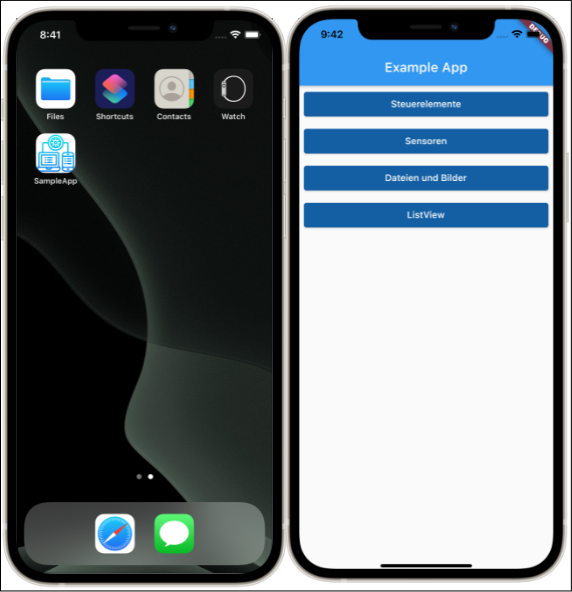
\includegraphics[width=\textwidth,keepaspectratio]{Images/Screenshot/Flutter1ios.png}
 \caption{Flutter App Screenshots I}
 \label{fig:FlutterAppI}
\end{figure}
 Sowohl der Name als auch das Launchericon der Anwendung sind korrekt übernommen worden.  Nach dem Start der Anwendung fallen jedoch Designabweichungen auf, die durch die Verwendung der Material Design Vorlagen in Flutter begründet sind.  Da der Compiler nicht,  wie in den Ausschlusskriterien festgelegt, den Style der Anwendung übersetzt,  entspricht das Ergebnis der Erwartungshaltung und ist,  weil daraus keine funktionelle Störung
entsteht,  an dieser Stelle akzeptabel.  Das zentrale Menü mit seiner Navigationsfunktion entspricht in der Ziel- dem der Testapp,  
unterscheidet sich jedoch,  wenn auch nicht in der Abbildung ersichtlich,  in der Animation. 
\newpage
Abbildung \ref{fig:FlutterAppII} stellt die Übersicht der Steuerelemente sowie die Werte der Smartphone-Sensoren dar.

\begin{figure}[!ht]
 \includegraphics[width=\textwidth,keepaspectratio]{Images/Screenshot/Flutter2ios.png}
 \caption{Flutter App Screenshots II}
 \label{fig:FlutterAppII}
\end{figure}
Die Übersicht der Steuerelemente stimmt  bezüglich der Verschachtelungen als auch der Funktionalitäten mit denen der Xamarin.Forms Variante überein,  was durch die Öffnung der Datums- und Uhrzeitauswahl validiert werden kann.  Ebenfalls korrekt übernommen wurde die Oberfläche der Sensorenansicht und alle Werte der Smartphonesensoren befinden sich im richtigen Format. Im Gegensatz zu der Xamarin.Forms App werden diese Daten jedoch nicht im gleichen Zyklus aktualisiert.  Dieser Unterschied basiert auf den Implementationen des jeweiligen Plugins und entsteht nicht durch den Übersetzer.  In der Xamarin.Forms App werden die Werte über Databindings geladen und mithilfe der \glq INotifyPropertyChanged\grq{} Schnittstelle wird die Benutzeroberfläche im Falle von Änderungen aktualisiert.  Diese Schnittstelle wurde in der Flutter Anwendung entfernt und der Teil des Quelltextes,  der Änderungen am \ac{ui} vornimmt mit einem Setstate-Block umschlossen,  damit sich die Oberfläche aktualisiert.  

Die in Abbildung \ref{fig:FlutterAppIII} dargestellten Screenshots zeigen ein Menü zur Arbeit mit Bildern, wobei der rechte zusätzlich den Berechtigungsdialog für die Kameraverwendung präsentiert. 
  
\begin{figure}[!ht]
 \includegraphics[width=\textwidth,keepaspectratio]{Images/Screenshot/Flutterios3.png}
 \caption{Flutter App Screenshots III}
 \label{fig:FlutterAppIII}
\end{figure}
Der Berechtigungsdialog entspricht nach Kompilierung in Darstellung und 
Funktion dem der Xamarin.Forms Version.  Auch der Zugriff auf die Kamera und die Galerie wurde, allerdings mithilfe der Erweiterung \glq image\_picker\grq , erfolgreich übersetzt.

Die Screenshots aus Abbildung \ref{fig:FlutterAppIV} visualisiert links die Galerie zur Bildauswahl und rechts die Darstellung der Benutzer in einer ListView.  


 \newpage 
\begin{figure}[!ht]
 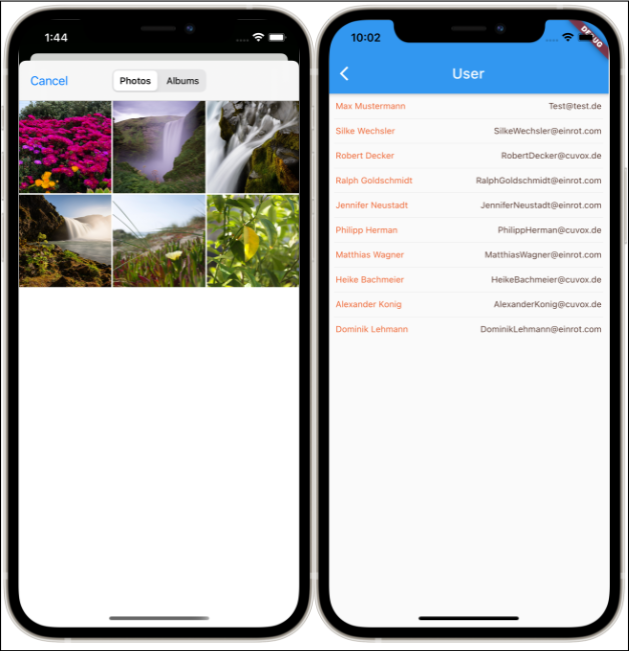
\includegraphics[width=\textwidth,keepaspectratio]{Images/Screenshot/Flutter4ios.png}
 \caption{Flutter App Screenshots IV}
 \label{fig:FlutterAppIV}
\end{figure}
Die korrekte Darstellung der \glq ListView\grq{} beweist, dass auch die Klassendefinition und ihr Konstruktor korrekt übersetzt wurden, denn nur unter dieser Voraussetzung konnte die Liste mit den  passenden Daten gefüllt werden.

Das Testobjekt konnte also vollständig überführt werden, was grundsätzlich die 
Funktionsfähigkeit des Prototypen beweist.  Bei einer Übersetzung aller in der Praxis möglichen 
Funktionalitäten von Xamarin.Forms bedarf es jedoch Erweiterungen des Compilers. 


